\chapter{Design} % You should concentrate on the more important aspects of the design. It is essential that an overview is presented before going into detail. As well as describing the design adopted it must also explain what other designs were considered and why they were rejected. The design should describe what you expected to do, and might also explain areas that you had to revise after some investigation. Typically, for an object-oriented design, the discussion will focus on the choice of objects and classes and the allocation of methods to classes. The use made of reusable components should be described and their source referenced. Particularly important decisions concerning data structures usually affect the architecture of a system and so should be described here. How much material you include on detailed design and implementation will depend very much on the nature of the project. It should not be padded out. Think about the significant aspects of your system. For example, describe the design of the user interface if it is a critical aspect of your system, or provide detail about methods and data structures that are not trivial. Do not spend time on long lists of trivial items and repetitive descriptions. You should also identify any support tools that you used. You should discuss your choice of implementation tools - programming language, compilers, database management system, program development environment, etc.

As has already been discussed, this project used a hybrid approach of a plan-driven methodology followed by an agile implementation. The design stage is where one methodology merges into the other.

A lot of time was invested in clarifying requirements, so that the common classes and methods could be established and fed into the initial design.

Certain design documentation, such as the database schema, was worth spending time creating and could be designed up front, since it was unlikely to change unless there was a change in requirements. Other things, such as class diagrams would not be suitable for upfront design, since the code would be refactored throughout the process and it would ultimately fall out of line with the documentation.

\section{Development choices}

\subsection{Programming language}

As a web-based solution, the options were somewhat constrained to server-side languages. PHP, Node and Ruby (on Rails) all came to mind. It was decided that PHP would be the most appropriate choice.

PHP is currently the most popular server-side programming language worldwide [REF], and, perhaps more importantly, it's the server-side language I have by far the most experience using. % http://w3techs.com/technologies/overview/programming_language/all

My philosophy was that, though I could have spent a few weeks learning the ins and outs of ASP.NET to deliver my project, it would be an unwise use of my time given that there was so much to build. I didn't want to find myself desperately trying to debug an obscure error in a new language a week before the deadline. 

Development experience aside, PHP being the most popular server-side language means that there is extensive support and documentation online: any problems faced during development have likely already been solved by other peoples' experiences. Moreover, if the project were to go open-source, it would be more likely to acquire a sizeable and active developer community than a more obscure language such as Go.

With my suite of Gherkin-syntax features, I needed a set of accompanying step definitions. The PHP de-facto standard implementation of BDD is Behat,  but after much lamenting on which BDD framework to use (see appendix~\ref{appendix:bdd}), it was decided that the project should use Ruby and Cucumber as its BDD framework.

\subsection{Reusing open-source software}

It was hoped that there would be an existing open-source ODR platform to base the project upon, upon which one would have been able to make the necessary modifications and extensions to support the maritime collision module, without having to build the entire platform from scratch, thereby being able to spend more time on the maritime law module.

Unfortunately, through fairly extensive research (see appendix ~\ref{appendix:choosingAFramework}), it was found that all of the existing ODR platforms are proprietary. Most ODR providers charge a subscription or one-off fee, be they service or platform providers. Given that they charge a fee, they'd be at a commercial disadvantage if they were to go open source.

Without an existing ODR platform to base the project upon, there was no option but to develop the core platform from scratch.

\subsection{Framework}

It makes sense to minimise development effort through the use of a framework, letting the combined efforts of thousands of contributing developers do the heavy lifting so that we are free to implement the application-specific code. Dozens of frameworks exist, so deciding on one can be difficult.

Large frameworks such as Zend and CakePHP are very constraining, requiring you to stick to their idea of what is the best development approach (specific directory structures, MVC design pattern, and so on) or else perform some very heavy, non-standard configuration to make it suit your project. Either of these heavyweight frameworks could be perfectly well suited to ODR, but generally speaking I try to stay away from non-transferable frameworks. I like to understand exactly how my application works, rather than delegate that understanding to a third-party library, and I like having the freedom to change frameworks painlessly at a later date - something which is not suited to heavyweight frameworks.

Lighter options exist: these include Huge, Opauth, Laravel and Fat-Free Framework. Huge looked promising to begin with but then appeared to be more of a middleweight framework, strongly encouraging certain directory structures. It would be a base that the ODR software would have to build upon, rather than a library that could be plugged into the system, only called as and when need.

Opauth looked nice and lightweight, but was aimed at projects which want to use OAuth for authentication, allowing people to sign in using their Twitter, Google, LinkedIn or Facebook account. This was not suitable, given our project requirements. Laravel was the next one considered and looked a little like PHP's answer to Rails, as it generates an entire application structure through a proprietary command.

Almost any one of these libraries would have been a suitable starting point. It would be impossible to thoroughly evaluate every framework to make a truly considered decision.

The most promising framework at first glance was Fat-Free Framework, or F3 as it is commonly known, having a low learning curve and an unconstraining nature. Its modular build meant that I could cherrypick the elements of functionality needed for the project, rather than go for an all-or-nothing installation. Interaction with the library is almost entirely through calls to namespaced classes. F3 is fundamentally different to its competitors because I could slot F3 into my code, rather than slotting my code into F3.

For similar reasons to my justification for my choice of PHP, I chose to use F3 due to the low learning curve and ability to get started quickly. I am more comfortable with native PHP than learning the ins and outs of a framework.

\section{Overall architecture}

The project can be broken down into three main components:

\begin{enumerate}
    \item \textbf{Core platform}, AKA SmartResolution. The majority of the project was spent developing this ODR software.
    
    \item \textbf{Maritime collision module}. This is a plugin for the SmartResolution software that defines a "Maritime Collision" dispute type and offers custom actions and business logic for these specialised cases.
    
    \item \textbf{SmartResolution Marketplace}, AKA smartresolution.org. 
\end{enumerate}

@TODO - highlight how different these are by describing the choice of licence for the core platform and for the maritime collision module, and why. e.g. maritime collision mod I wanted people to be able to download and modify as a basis for their own modules, if this were GPL they'd be obliged to release the source etc.

Chose GPL for SmartResolution because (compared to Wordpress' GPLv2) nobody should be able to download, modify and then redistribute the core software under another brand (or at least a closed source brand). (@TODO - double-check OS license terms).

\subsection{Core platform}

SmartResolution [REF] is the ODR platform offering the core online dispute resolution requirements, such as organisation and user registration, dispute creation, messaging, file uploads, and so on. It offers the minimum facilities necessary to successfully negotiate a dispute online.

As this will be the basis of all the other components, it should also be the most thoroughly engineered, backed up with integration and unit tests, continuous integration, automated code quality checks and dependency status checks.

\subsection{Maritime collision module}

This module is separate from the core platform and lives in its own repository [REF]. It can be installed to any SmartResolution installation by being deployed to the top-level "modules" directory; no further configuration is required.

As discussed in the background and initial requirements, it was intended for this to be a feature-rich module that could find similar historic cases, cross-check agents' answers with maritime law, and approximate the likelihood of an agent's success in court. This is still theoretically possible. However, given the lack of time and resources, this is more of a prototype; a teasing glimpse as to what might be possible given a few more development hours.

\subsection{SmartResolution Marketplace}

This is the vendor site for SmartResolution, explaining what SmartResolution is and offering a download link to a production-ready version. Its subdomain, demo.smartresolution.org, has a live demo of the SmartResolution software installed so that users can try out the software before they download. However, the main purpose for smartresolution.org is the \emph{Marketplace} facility.

\section{WordPress: a comparison}

The commercial viability of the software (discussed in appendix~\ref{appendix:commercialViability}) drew some parallels with the blogging software WordPress. They could be said to have a three-tier system:

@TODO represent with a diagram? Pyramid?

\begin{enumerate}
    \item \textbf{WordPress platform}: blogging software that can be downloaded, installed and hosted on your own server.
    
    \item \textbf{WordPress plugin}: a self-contained package that can be installed to a WordPress installation and augment the core installation with additional functionality.
    
    \item \textbf{Plugin Directory}: a searchable area of the WordPress.org website, accessible directly through your own WordPress installation, allowing the painless and automatic installation of plugins. This facility is tightly coupled to the administrative functions in the core software. Administrators are able to browse, download and install plugins from wordpress.org, from within the WordPress installation itself. % https://wordpress.org/plugins/
\end{enumerate}

@TODO - some discussion about the components of my project and why they're similar to this.

\section{Design: SmartResolution}

\subsection{Database schema}

\begin{figure}[h!]
  \centering
    \ifimages
    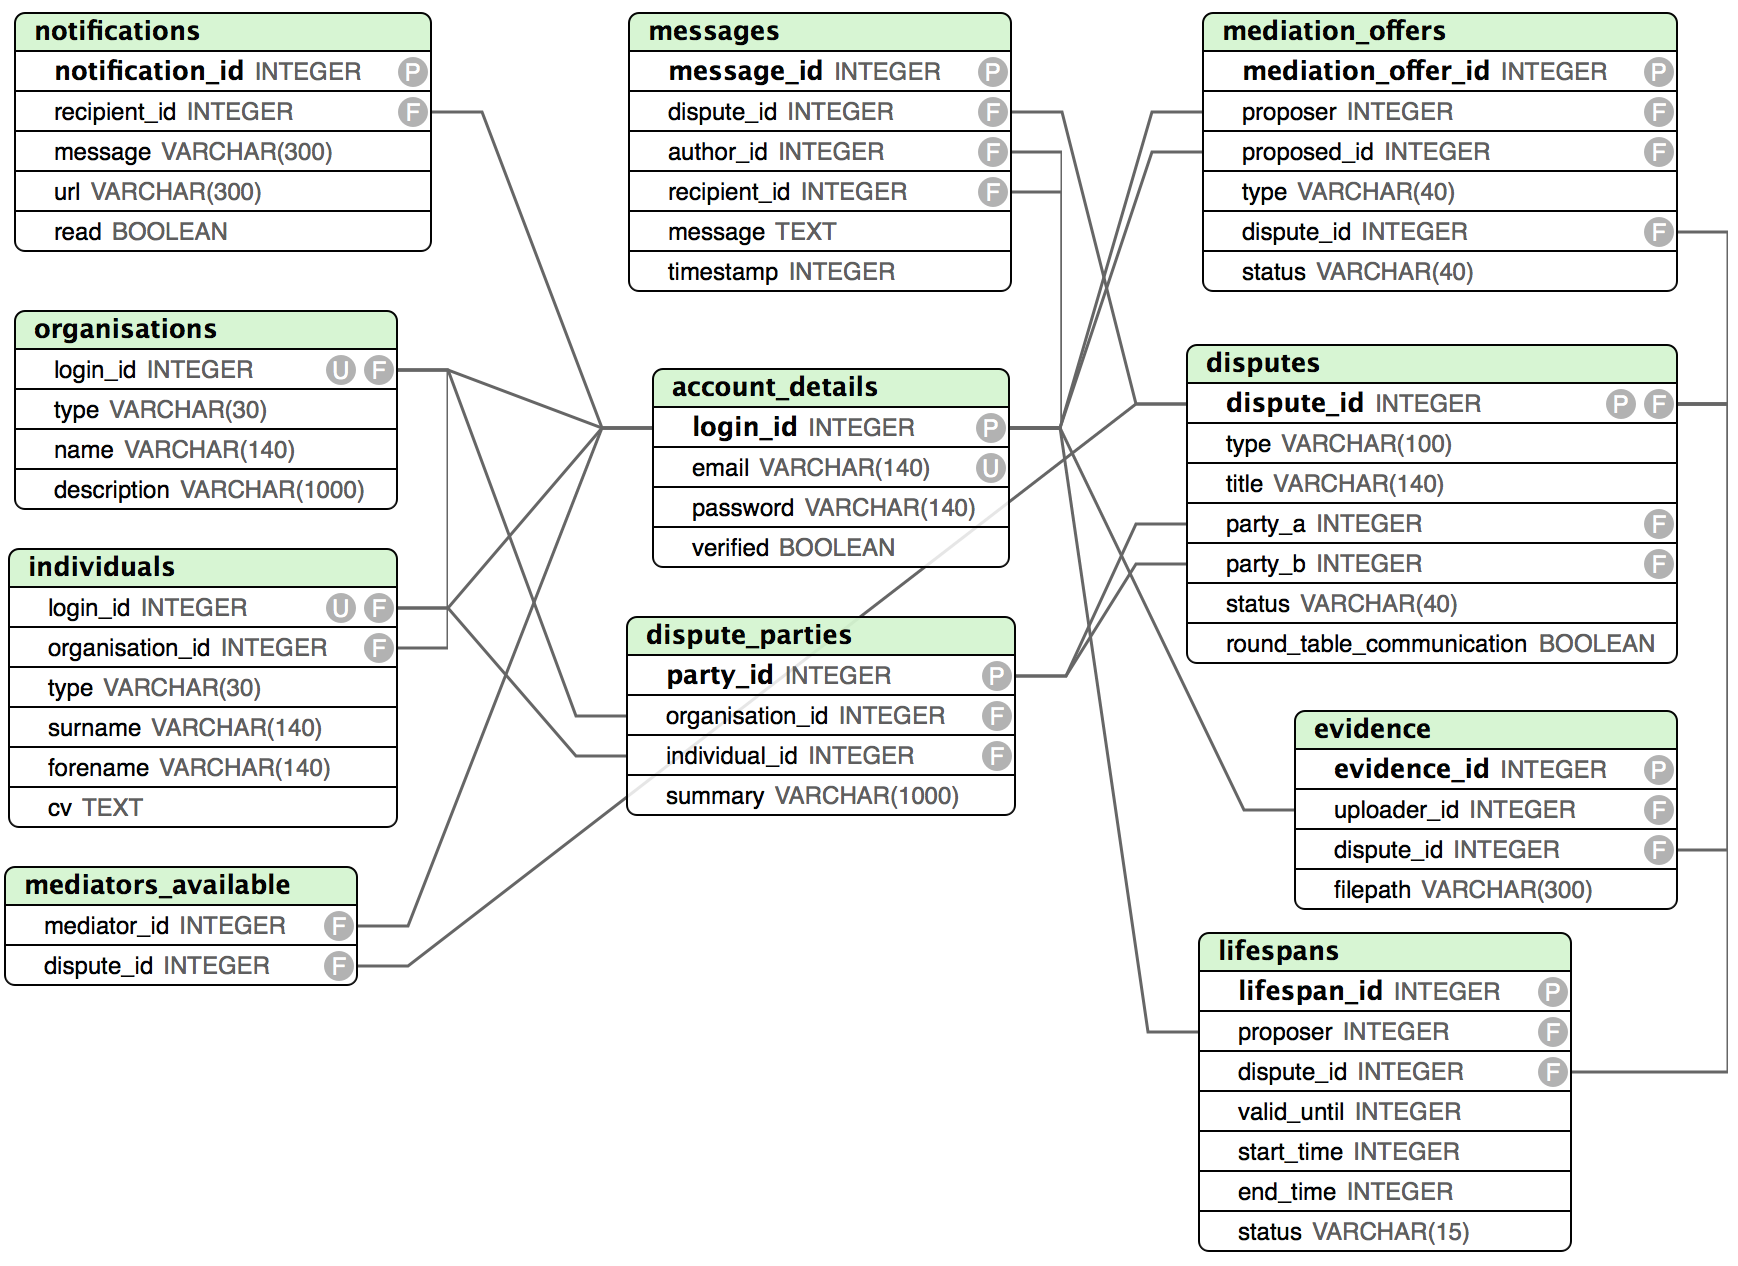
\includegraphics[width=\textwidth]{database}
    \fi
  \caption{Database schema for the SmartResolution core platform}
  \label{uml:databaseSchema}
\end{figure}

Figure~\ref{uml:databaseSchema} shows the database schema for the SmartResolution core platform, where \lstinline{P} symbols refer to primary keys, \lstinline{F} symbols refer to foreign keys, and \lstinline{U} symbols refer to unique integrity constraints. Lines generally denote where one table key references another, i.e. a foreign key visualisation.

For a full explanation and justification of the database design, please refer to appendix~\ref{appendix:database}.

\subsection{Module support}

This section of work is separate from the maritime collision module work, and is concerned with how the core platform should support modules at an abstract level. There should be no maritime-collision-specific code in the core SmartResolution platform, but the platform must support all functionality required by the module.

Taking inspiration from WordPress' Plugin API, the project uses the concept of 'hooks'. WordPress fires events at various points throughout the normal running of a WordPress installation; these events can be subscribed to and a custom function executed to achieve some arbitrary purpose.

Below is the \lstinline{add_filter} function as an example [REF]: %http://codex.wordpress.org/Function_Reference/add_filter

\begin{lstlisting}
add_filter('img_caption_shortcode', 'my_img_caption_shortcode_filter',10);
\end{lstlisting}

The first argument is the event to listen for, the second argument is the custom function to execute, and the third argument is an integer denoting the priority of our subscription (where a higher integer means our custom function is executed before the functions of lower-priority subscribed plugins).

F3's routing API [REF] can extend this concept further:

\begin{lstlisting}
$f3->route('GET /some-route' => 'MyClass->handler');
\end{lstlisting}

F3's routing allows the developer to assign handling to a public method of a class, rather than a global function, keeping the codebase namespaced and tidy.

These principles formed the basis for the design of the module support:

\begin{lstlisting}
on('event', 'function_to_call', 'priority');
\end{lstlisting}

\subsection{Exposing other methods}

An event-subscription mechanism can only get you so far. One needs to be able to manipulate the rendered output of SmartResolution, for example adding an item to the dashboard of a dispute.

This could be accomplished by interacting with the core platform, as in the example below.

\begin{lstlisting}
global $dashboardActions;
$item =  array(
    'title' => $params['title'],
    'image' => $params['image'],
    'href'  => $params['href']
);
array_unshift($dashboardActions, $item);
\end{lstlisting}

However, this encourages tight coupling between the module and the underlying platform, locking the core platform into a particular design and risking breaking backwards compatibility should SmartResolution be refactored in the future. For example, if the \lstinline{$dashboardActions} global variable was removed from the core platform, or the dashboard actions represented with something other than an array, it could break any existing modules relying on that specific implementation.

Again, WordPress provided inspiration for the design. WordPress exposes a number of global functions, e.g. \lstinline{get_the_id}, which gets the ID of the current post. [REF] %https://codex.wordpress.org/Function_Reference/get_the_ID

So, the core platform was extended to create a number of global functions. [REF] One could now manipulate the rendering of the dashboard like this: % http://smartresolution.org/module-docs/index.html

\begin{lstlisting}
dashboard_add_item(array(
    'title' => 'Some Action',
    'image' => get_module_url() . '/images/icon.png',
    'href'  => get_dispute_url() . '/custom-route'
));
\end{lstlisting}

This is much cleaner and easier from the module developer's perspective. It was always important that there should be as few barriers as possible when it comes to module development, if developers are to get excited about SmartResolution.

\subsection{Module persistence}

This was the most difficult area to tackle, as it raises important security issues. Whereas hooking into events and changing the rendering could break aspects of the SmartResolution functionality if the developer is not careful, these are usually temporary and reversable. Interacting with the database, however, introduces persistent changes and can do much more damage.

If the system allowed arbitrary SQL queries and an uncareful developer accidentally executed a \lstinline{DROP TABLE} statement, all manner of data could be lost. This isn't so important on a small demo site with three or four registered users, but if SmartResolution were ever used on a large-scale website, the result could be catastrophic.

On the one hand, the system has to trust developers. Regardless of the database access explicitly exposed, there's nothing stopping a developer from running PHP's \lstinline{shell_exec} function [REF] and executing any command they wish. Also, in terms of the database interaction, there's nothing stopping developers from accessing the global \lstinline{DB} class used by the core platform, especially since this is open source and the developer can easily find out how to access it.

The system should trust developers, but it should not trust developers to write perfect code. Though most developers would use an arbitrary-SQL-execution ability only for querying the database for a legitimate reason, they may expose a vulnerability if not thoroughly tested. If their SQL query takes a user input - for example, if they're writing a search engine module - and they don't sanitise the query, then they're letting the \emph{end user} run arbitrary SQL. The end user doesn't necessarily have the best interests of SmartResolution at heart.

With security in mind, it was decided that the global function definitions should be expanded to define functions supporting specific SQL interactions, e.g. creating tables, selecting rows, updating records, and so on. Early on it was tempting to allow table schema updates on the fly, creating columns as and when they were needed, but this felt dangerous and was tricky to implement. So I started off proceedings with a \lstinline{declare_table} function:

\begin{lstlisting}
declare_table('my_table', array(
    'a_text_field' => 'TEXT NOT NULL',
    'an_int_field' => 'INTEGER DEFAULT 0',
    'initiated'    => 'BOOLEAN'
));
\end{lstlisting}

This could then be inserted into and queried using specific, named functions. This does somewhat restrict what the developer can do - for example, there is no method for doing SQL table joins - but more often than not, the developer can still achieve what they need to achieve using pure application code.

In the above example, \lstinline{my_table} is not the name of the created table. Instead, it is namespaced as \lstinline{module__[module_name]__my_table}. The module developer doesn't need to know this, and can continue to refer to \lstinline{my_table} in all of their queries as if that is the name of the table. This means we have the advantage of namespacing our tables (preventing duplicate table names between modules for common table names, e.g. "config") but without the technical overhead of having to rememember to prefix table names with that namespace.

Most modules will require some sort of persistence layer to be useful, but developers are not necessarily locked into this database setup. They can use PHP's \lstinline{shell_exec} command to create a new SQLite database in their module's directory, giving them complete freedom (and the responsibility it comes with). Or, they can use PHP's \lstinline{file_put_contents} to save to a file, perhaps in conjunction with \lstinline{json_encode} to save a PHP array as a JSON file. The database functions I offer cut out some of the complexity of doing this from scratch.

\section{Design: SmartResolution Marketplace}

Early versions of SmartResolution used a PHP array to describe which modules were installed and which were active. [REF] % https://github.com/ChrisBAshton/smartresolution/blob/6287211d49006e87a8d2035906eb58da22217906/webapp/modules/config.php 

A more user-friendly solution was the creation of an admin dashboard: the ability to sign into an administrator account on your SmartResolution instance, view the installed modules, and activate/deactivate them through a user interface. Following on from this is the ability to view a list of modules, pulled in from SmartResolution.org, and download and install them directly through SmartResolution, like WordPress does with plugins.

To accomplish this, there is a JSON feed of featured modules on smartresolution.org. [REF] %http://smartresolution.org/marketplace/feed

This feed is pulled in and converted to HTML, both directly on the marketplace itself [REF] and the SmartResolution admin marketplace dashboard option, emulating what WordPress does with its modules (which are viewable both through your own installation of WordPress and on WordPress itself [REF]). %http://smartresolution.org/marketplace
%https://wordpress.org/plugins/

Defining featured and "other" modules externally on smartresolution.org gives the SmartResolution maintainers the freedom to change the contents of that JSON, and therefore change which modules are presented to administrators of SmartResolution instances, regardless of when the instance was installed. This presents a commercial opportunity, as hinted by the "Coming soon" modules for Divorce and Breach of Contract, which needn't necessarily be downloaded for free.

@TODO move to evaluation? :

The process for putting a module on the SmartResolution Marketplace is currently manual. This is something I would want to automate in the future, for example by taking a GitHub repository URL and zipping up the contents automatically. However, this manual process does at least give me the option to check the code and make sure there is nothing insidious about its contents before making it available on the marketplace.

The admin dashboard feature was one of the last to be added. Figure~\ref{uml:databaseSchema} shows the \lstinline{administrators} table, which requires nothing more than the \lstinline{login_id} associated with an \lstinline{account_details} entry.

Currently, the admin account must be created manually in the database. In future, this would be a part of the installation process, prompting the user for an admin email and password.

With the admin account created, the admin can log into their account to be presented with three options: Marketplace, Modules and Customise. The latter option is a placeholder and contains no functionality. It is hoped that this might later allow the admin to customise their instance, e.g. by changing the SmartResolution logo, enabling/disabling mediation, and so on.

The other two options are fully functional. The `Marketplace' converts the modules JSON feed into a HTML page, detects if the module is already installed on the instance, and if not, provides an option to download and install the module in one button press.

The `Modules' option lists all of the installed modules and whether or not they are active. From this screen, the admin can activate, deactivate or delete the module from their SmartResolution instance.

There is one more admin feature I'd have liked to have added given more time: the ability to switch themes. WordPress allows bloggers to easily change the look and feel of their site by activating a new theme. This is something that is perfectly possible in SmartResolution too, thanks to its MVC architecture.

\section{Design: Maritime collision module}

As discussed in the requirements section, the basis for the business logic in this module would be the Convention for the Unification of Certain Rules of Law with respect to Collisions between Vessels. Everything that is required to apply the Convention can be gathered from a few simple questions, visualised in the flowchart in figure~\ref{uml:maritimeLogic}.

\begin{figure}[h!]
  \centering
    \ifimages
    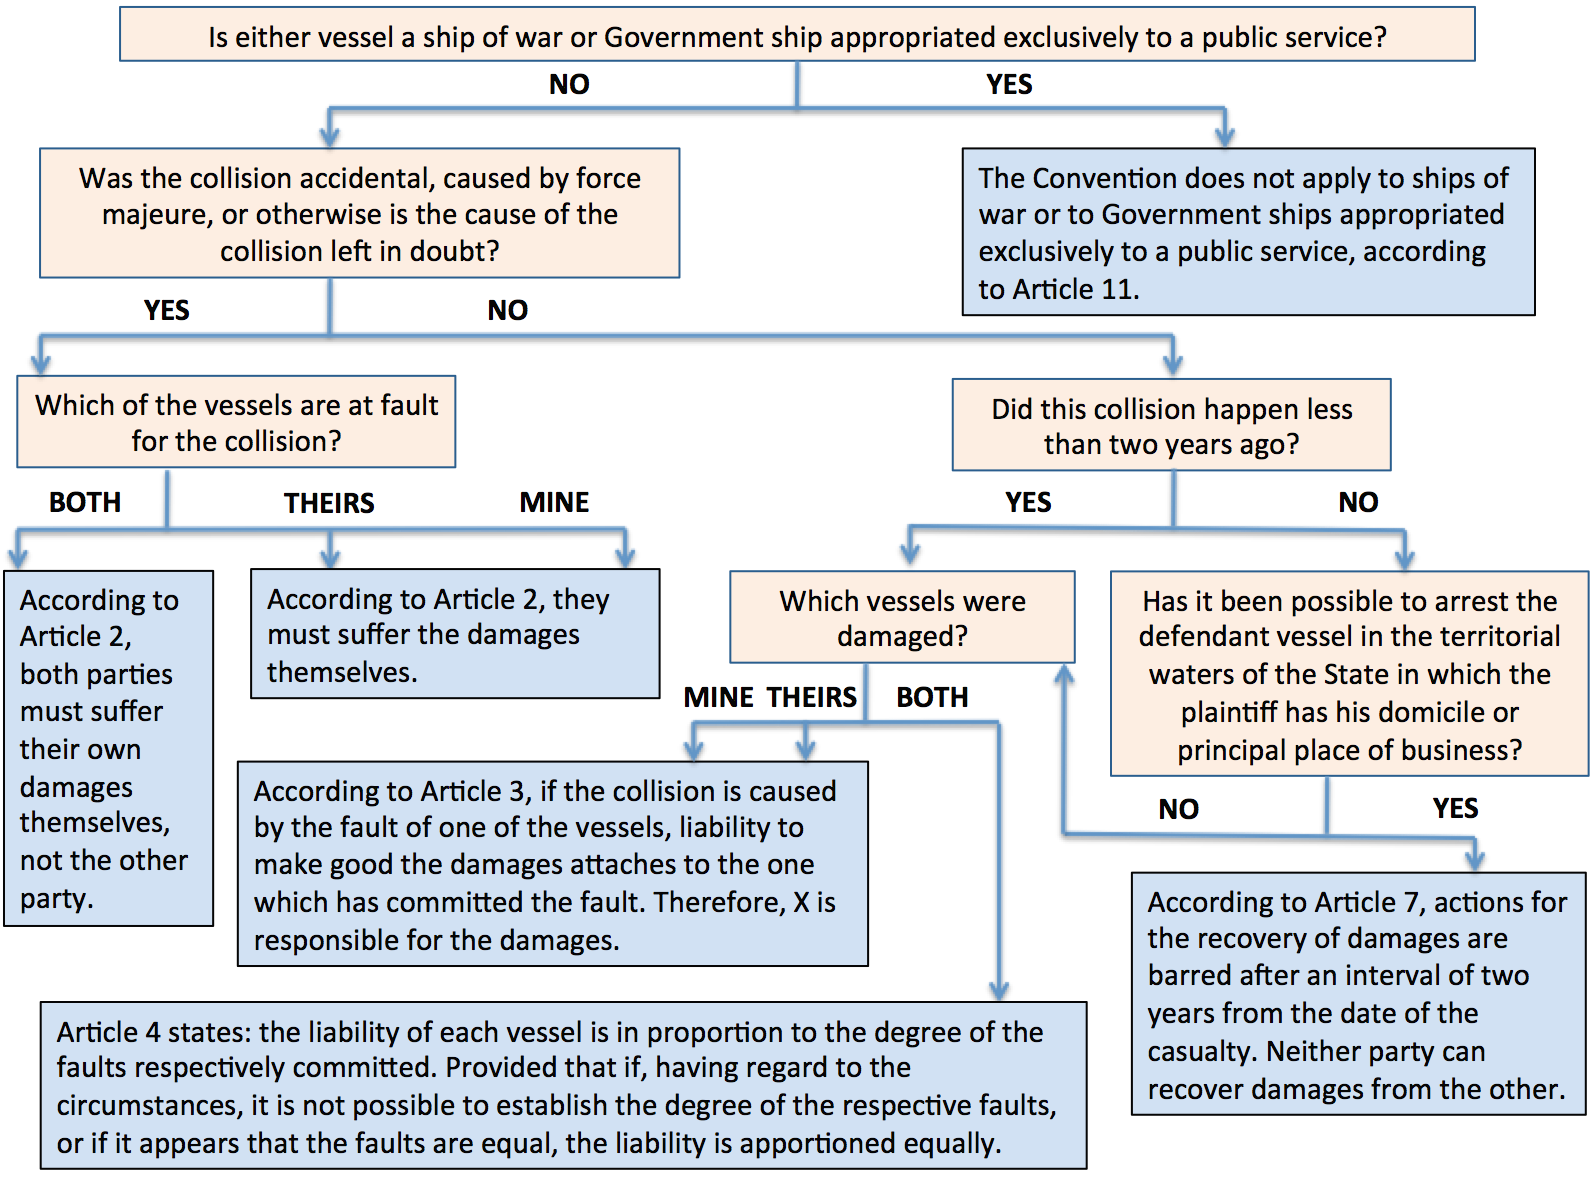
\includegraphics[width=\textwidth]{maritime_collision_logic}
    \fi
  \caption{Logic for Maritime Law results}
  \label{uml:maritimeLogic}
\end{figure}

Some of the business logic could be encapsulated in the JSON representing the questions. For example, some questions should only be displayed if certain prerequisites are satisfied. The questions are represented in the following format:

\begin{lstlisting}
    {
        "prerequisites": [
            {
                "question_id":     "article_11",
                "required_answer": "no"
            }
        ],
        "id":   "article_1",
        "text": "Which vessels were damaged?",
        "type": "select",
        "options": [
            {
                "text" : "The vessel of my client",
                "value": "mine"
            },
            {
                "text" : "The vessel of the other party",
                "value": "other"
            },
            {
                "text" : "Both vessels",
                "value": "both"
            }
        ]
    }
\end{lstlisting}

In the above example, the question whose id is \lstinline{article_1} (corresponding to Article 1 of the Convention) is only displayed if the agent answers the question whose id is \lstinline{article_11} with the answer "no".

This module was developed in tandem with the module support in the core platform. As such, it uses most of the events and hooks exposed by the platform.

When the agents have answered all of the relevant questions, the following happens:

\begin{itemize}
    \item The answers are compared to make sure they tally. If one agent says both vessels were damaged and the other agent says only their vessel was damaged, the answers do not correspond and a conclusion cannot be reached. The module cannot be expected to cope with conflicting information. The module would inform the agents of this.
    \item Provided both answers correlate, the module's ResultsCalculator class calls the deduceSummary() method [REF], which contains the hard-coded maritime law logic. A resolution is then presented to the agents.
\end{itemize}

Due to the lack of time the resulting module is a little simplistic, but the point is that the core platform supports any arbitrary module. Modules can be as big and complex as time allows.

\section{User interface}

Bootstrap was used to set up much of the initial design defaults and as a basis for the layout, wanting a clean and attractive look but not wanting to spend too much time on the user interface. Another advantage of using Bootstrap as a UI framework is that the theme is fully responsive by default.